\documentclass[11pt,a4paper]{article}
\usepackage[utf8]{inputenc}
\usepackage[T1]{fontenc}
\usepackage{lmodern}
\usepackage{upgreek}
\usepackage[slovene]{babel}
\usepackage{color}
\usepackage{graphicx}
\usepackage{verbatim}
\usepackage{amsmath}
\usepackage{float}
\usepackage{xcolor}
\usepackage{todonotes}
\usepackage{listings}
\usepackage{fullpage}
\usepackage{xparse}
\usepackage{icomma}
\usepackage[backend=bibtex]{biblatex}
\addbibresource{viri.bib}
\usepackage[title]{appendix}

% code styling
\lstset{language=Python,keywordstyle={\bfseries \color{blue}}}
\NewDocumentCommand{\codeword}{v}{%
	\texttt{\textcolor{blue}{#1}}%
}
\DeclareMathOperator{\Hz}{Hz}
\DeclareMathOperator{\kHz}{kHz}

\begin{document}

\title{Osnovna karakterizacija senzorja Sharp GP2Y1010AU0F za opazovanje koncentracije aerosolov v zraku}
\author{"Ziga Pata"cko Koderman$^1$ \and Klemen Bu"car$^2$}
\date{%
  $^1$FMF, Oddelek za fiziko, Univerza v Ljubljani\\
  $^2$Institut Jožef Stefan, Ljubljana\\[3ex]
  Izdaja: Ljubljana, \today
}

\maketitle
\thispagestyle{empty}

\begin{center}
IJS delovno poro"cilo\\ IJS-DP-xxxxxx
\end{center}

\tableofcontents
\pagebreak

\section{Uvod}
\todo{prvo stran moram "se dokoncati}

Cilj projekta je razviti cenovno ugoden sistem za opravljanje meritev koncentracije trdnih delcev v zraku ter oceniti njegovo negotovost. Za ta namen je bilo izbrano tipalo GP2Y1010AU0F podjetja Sharp \cite{sharp-gp2y1010au0f}. To je opti"cni senzor, ki za delovanje izkori"s"ca odvisnost med koli"cino sipane svetlobe pri potovanju skozi medij in koncentracijo delcev.

\vspace{3cm}
\begin{figure}[H]
	\begin{center}
		\includegraphics[width=10cm]{setup_view.jpg}
		\caption{Raspberry Pi s priklju"cenim tipalom Sharp GP2Y1010AU0F}
		\label{setup-view}
	\end{center}
\end{figure}

\pagebreak

\section{Tipalo Sharp GP2Y1010AU0F}

Tipalo Sharp GP2Y1010AU0F \cite{sharp-gp2y1010au0f} sestavljata infrarde"ca LED, ki v pulzih emitira IR svetlobo, ter fototranzistor za detekcijo sipane svetlobe. Oba sta zaprta v ohi"sje in postavljena v kota ob isti stranici tako, da svetloba iz diode ne prehaja neposredno na fototranzistor (slika \ref{sensor-scheme}). Meritev opravimo tako, da LED vklopimo s kratkim pulzom preko RC vezja ter opazujemo odziv fototranzistorja, ki je posledica:
\begin{itemize}
	\item odboja svetlobe od notranjih sten ohi"sja in
	\item sipanja svetlobe pri potovanju skozi medij.
\end{itemize}

\begin{figure}[H]
	\begin{center}
		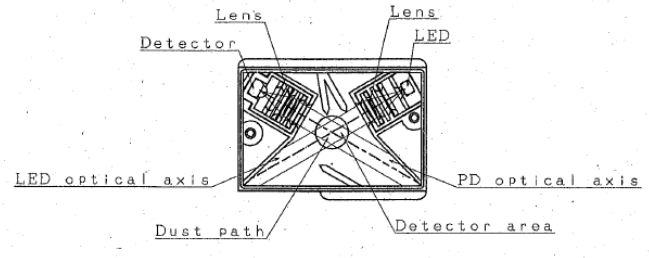
\includegraphics[width=12cm]{sensor-scheme.png}
		\caption{Skica tipala GP2Y1010AU0F}
		\label{sensor-scheme}
	\end{center}
\end{figure}

Proizvajalec tipala priporo"ca, naj za pro"zenje IR LED uporabimo RC vezje z 220\,$\mu$f kondenzatorjem in 150\,$\Omega$ uporom \cite{sharp-gp2y1010au0f}. Karakteristi"cni "cas takega vezja je

$$
\uptau = RC = 0,033\,s
$$

Po vsakem pulzu LED moramo vezje spet napolniti, za kar porabimo nekaj karakteristi"cnih "casov. Predpostavimo, da trije karakteristi"cni "casi zadostujejo.

$$
\nu = \frac{1}{t_0} \approx \frac{1}{3 \uptau} = 10\,\Hz
$$

Meritve lahko torej opravljamo s frekvenco najve"c 10\,Hz. RC vezje nam s tem prepre"cuje, da bi LED preobremenili s tokom.

Po vsakem pulzu LED opazujemo odziv fototranzistorja. To je napetostni impulz, ki ga vzor"cimo z 10-bitnim ADC (ang. \textit{analog to digital}) pretvornikom MCP3002 \cite{mcp3002}, in dobimo njegovo digitalno obliko.

\begin{figure}[H]
	\begin{center}
		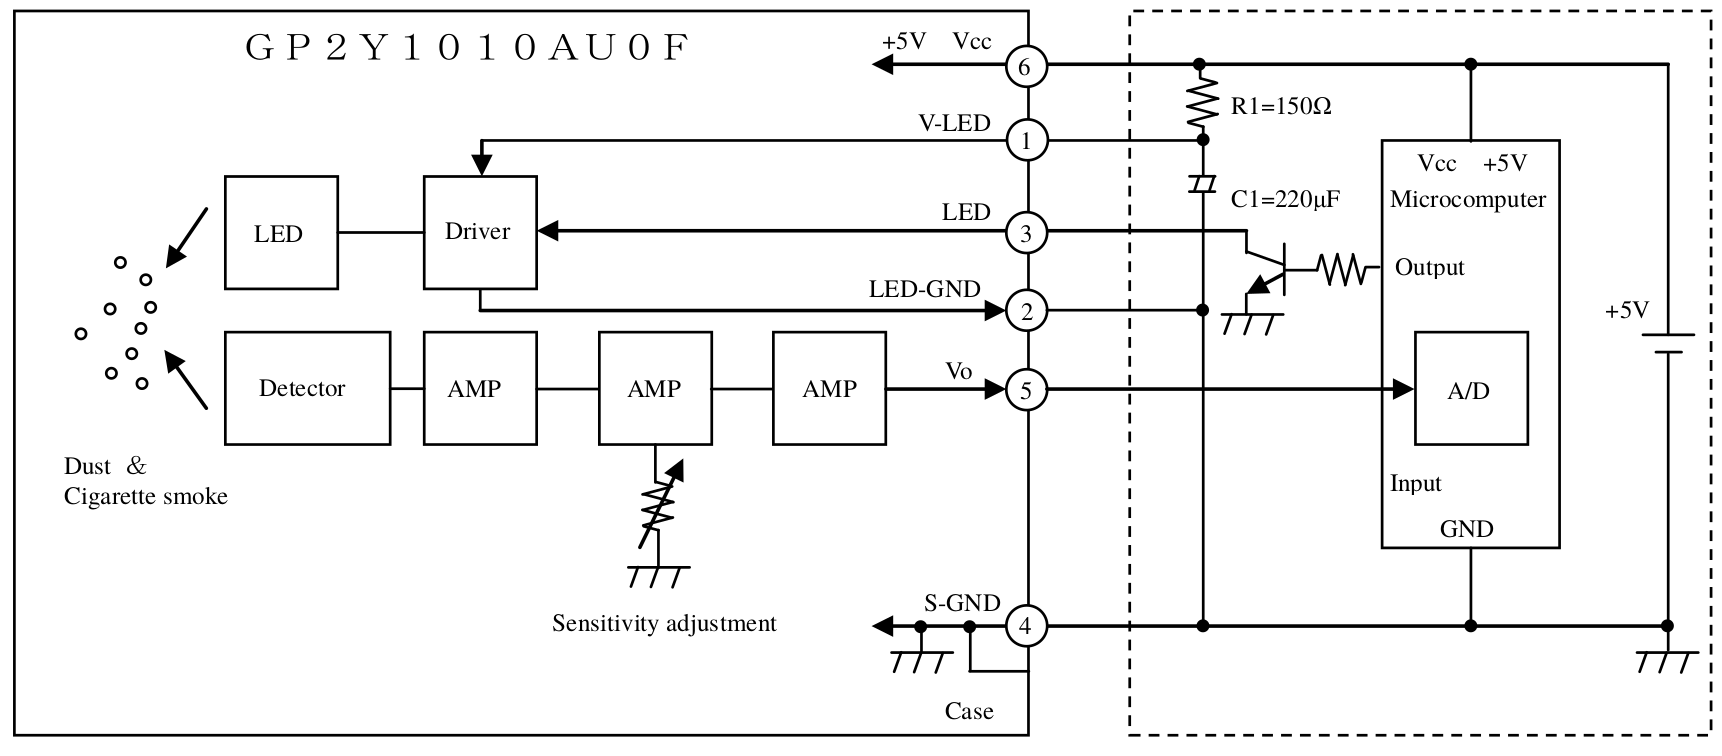
\includegraphics[width=12cm]{integration-scheme.png}
		\caption{Primer priklopa tipala}
		\label{integration-scheme}
	\end{center}
\end{figure}

Celoten proces, ki zajema:
\begin{itemize}
	\item krmiljenje infrarde"ce LED,
	\item branje pretvorjenega signala in
	\item shranjevanje meritev,
\end{itemize}

krmili mikrora"cunalnik Raspberry Pi \cite{rbpi-wiki}. Meritvam pripi"semo tudi datum in "cas merjenja. V ta namen uporabimo "se RTC (ang. \textit{real time clock}) modul, saj Raspberry Pi sam tega nima.


\begin{figure}[H]
	\begin{center}
		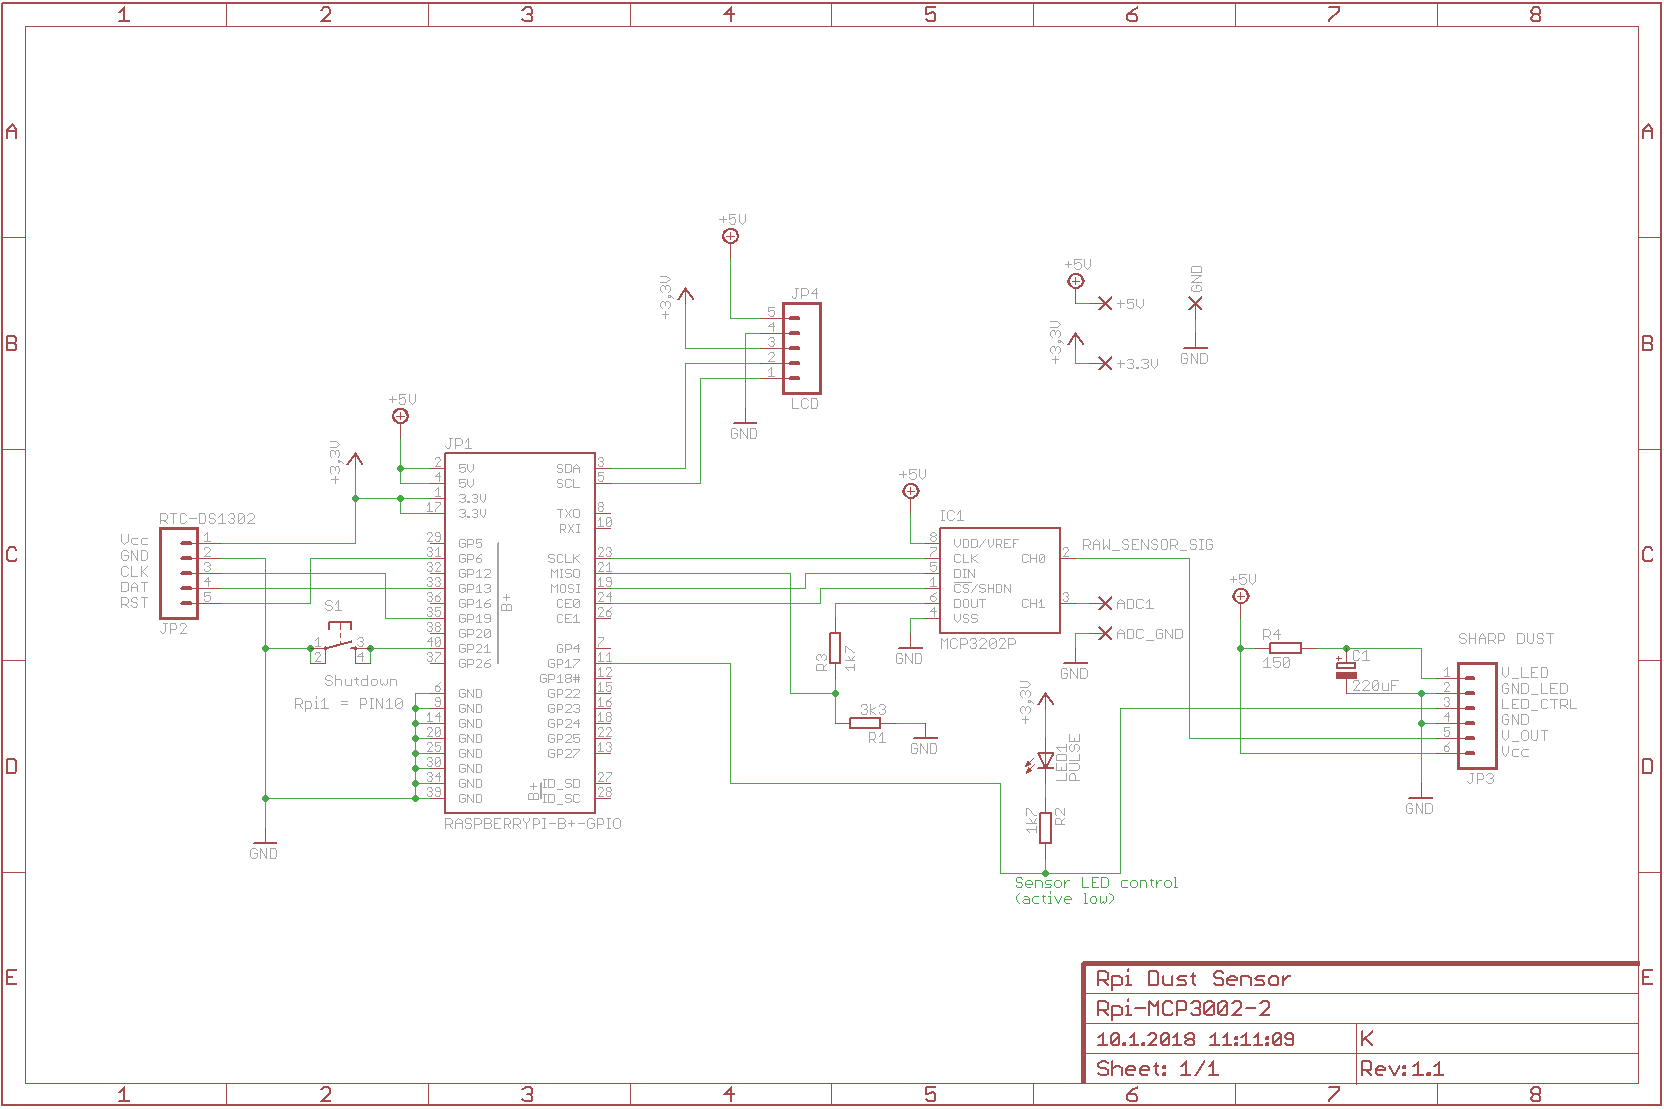
\includegraphics[width=12cm]{scheme.png}
		\caption{Shema vezja}
	\end{center}
\end{figure}

Prebrani pulz vzor"cimo s frekvenco $ \approx $ 35,7\,kHz (kolikor zmore Raspberry Pi) ter ga shranimo kot mno"zico 50 to"ck, v tabelo znotraj HDF5 datoteke \cite{hdf5}.

Proizvajalec priporo"ca, da napetost na fototranzistorju od"citamo 0,28\,ms po vklopu LED. Kljub temu na"s sistem zajema odziv fototranzistorja 1,4\,ms od vklopa LED. "Cas 0,28\,ms sovpada z vrhovi izmerjenih pulzov, tako da predvidevamo, da v resnici i"s"cemo vrh pulza. 

\begin{figure}[H]
	\begin{center}
		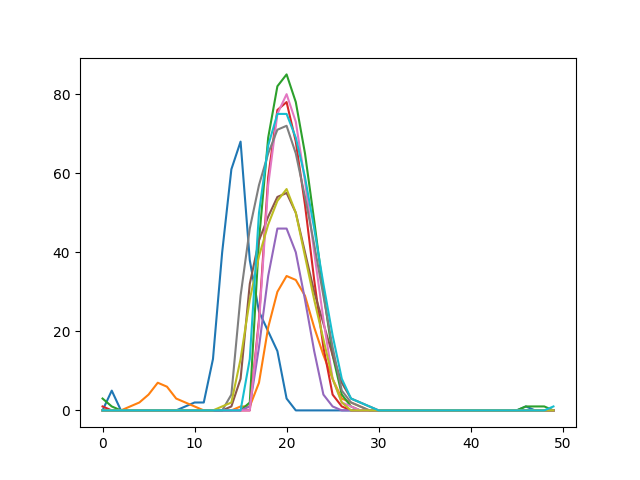
\includegraphics[width=12cm]{pulses_old.png}
		\caption{Primer 10 odzivov fototranzistorja pri vzor"cenju 50 to"ck}
		\label{pulses-old}
	\end{center}
\end{figure}

S slike \ref{pulses-old} je razvidno, da vzorci pulzov med seboj niso preve"c podobni. Vrhovi so zelo razpr"seni in odstopajo za $ \approx \pm $ 40\,\%.

\clearpage

\section{Izhod iz tipala}
Zaradi neuporabnosti obstoje"cih meritev se odlo"cimo za sistemati"cno analizo in nadgradnjo obstoje"cega sistema za zajem in analizo vzorcev.

\subsection{Neenakomerno vzor"cenje}
Zaradi variabilne obremenitve procesorja na krmilniku Raspberry Pi dobi proces za zajemanje meritve spremenljivo koli"cino procesorskega "casa. To"ck na pulzu torej ne od"citavamo z enakomerno frekvenco. Odstopanja odpravimo tako, da vsaki to"cki dodamo "casovni "zig.

\begin{figure}[H]
	\begin{center}
		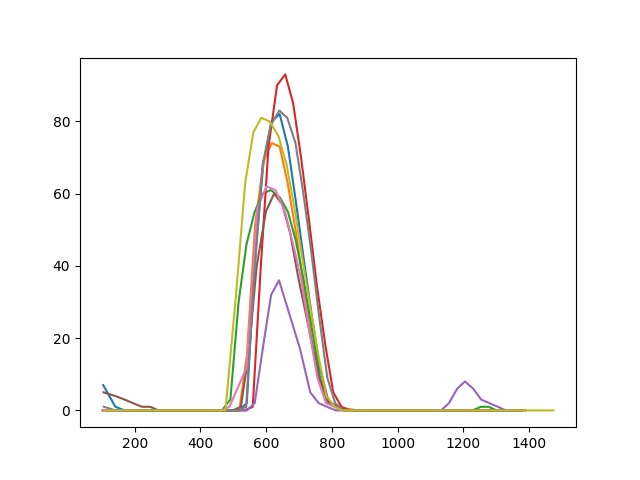
\includegraphics[width=12cm]{aligned.png}
		\caption{Pulzi po "casovni poravnani izmerjenih to"ck v $\mu$s}
		\label{aligned}
	\end{center}
\end{figure}

Ko to"cke poravnamo relativno na "cas v"ziga LED, opazimo precej lep"so poravnavo vrhov (slika \ref{aligned}).

\subsection{Velikost vzorca}
Pri opravljanju meritve ne poznamo natan"cnega pretoka zraka skozi tipalo. Zana"samo se na konvekcijsko gibanje zraka. Da preverimo, ali to zadostuje za potrebe meritve, pretok prisilno pove"camo z ventilatorjem ter opazujemo morebitne spremembe. Ne opazimo nobenih sprememb ter sklepamo, da je konvekcijski pretok zraka dovolj"sen.

\subsection{Svetlobne motnje iz okolice}
Ohi"sje tipala je odprto, da lahko skozenj te"ce zrak. To pa fototranzistor v tipalu izpostavi zunanjim svetlobnim virom. Ti lahko na meritve vplivajo v obliki "suma ali sistemati"cne napake (na primer razlika med dnevom in no"cjo). To preverimo s postavitvijo tipala v popolno temo. Opazimo, da so vrhovi pulzov poravnani bistveno bolje (slika \ref{dark}). Meritve od tu naprej opravljamo v temi.

\begin{figure}[H]
	\begin{center}
		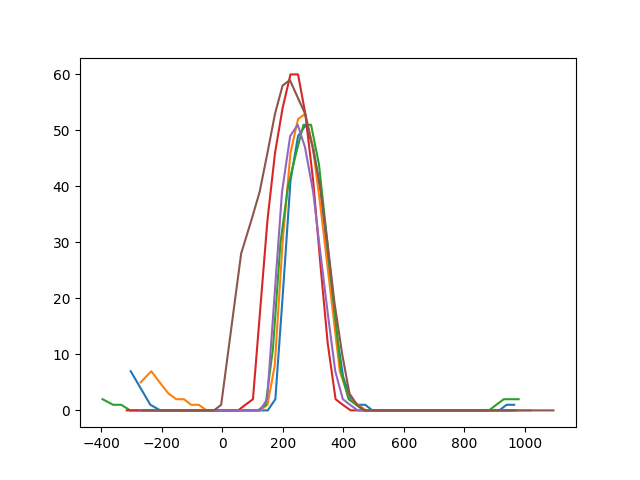
\includegraphics[width=12cm]{dark.png}
		\caption{Pulzi, izmerjeni v temi v $\mu$s}
		\label{dark}
	\end{center}
\end{figure}

\subsection{Dolo"canje vrha}
Do zdaj smo pri zajemanju podatkov za vrh pulza vzeli kar najvi"sjo izmerjeno to"cko. Ta pa zaradi premajhne frekvence vzor"cenja nikoli ne sovpada popolnima s pravim vrhom. Napako odpravimo z napenjanjem parabole na najvi"sjih nekaj to"ck. Vsak pulz zajema pribli"zno med 10 in 20 to"ck, tako da se odlo"cimo za napenjanje parabole na najvi"sjih 7.

\subsection{Meritve v vakuumu}
Navkljub vsem izbolj"savam meritve ostajajo polne "suma. Da bi to kvantificirali, postavimo tipalo v vakuum ter popolno temo. S tem "zelimo odstraniti vse zunanje dejavnike ter izmeriti izklju"cno odboj svetlobe od ohi"sja. Napaka meritve v tem primeru prihaja iz negotovosti pri od"citavanju ter neenakomernih pulzov LED.

Razlike med meritvami na prostem in v $ 15mbar $ vakuumu ne zaznamo. Sklepamo, da potrebujemo "se ni"zji pritisk.

\subsection{Analiza podatkov}
Analiza podatkov poteka na lo"cenem ra"cunalniku in ni del naprave za opravljanje meritev. Obstoje"ci sistem za obdelavo meritev povpre"ci vi"sine vrhov pulzov v "zelenem "casovnem obdobju (nekaj 10 minut). Rezultate skupaj z meritvami, opravljenimi z merilnikom Grimm mini-LAS, nari"se na graf. Posebne korelacije ne opazimo. Da bi to kvantificirali, korelacijo tudi izra"cunamo. Ta je majhna - za ve"cino en dan trajajo"cih meritev je njena vrednost pod 0,5, kar ni uporabno.

\subsubsection{Knji"znica za obdelavo podatkov}
Za hitrej"so in la"zjo analizo podatkov je bilo ve"c manj"sih programov zdru"zenih v Python knji"znico po imenu \codeword{Analysis}. Ta je zelo prilagodljiva in uporabniku omogo"ca nalaganje podatkov o pulzih iz hdf5 \cite{hdf5} datotek in risanje grafov s samo nekaj ukazi.

Obdelava velike koli"cine podatkov (v"casih tudi za ve"c dni) je zelo dolgotrajna. Knji"znica \codeword{Analysis} je zato optimizirana z uporabo knji"znice \codeword{NumPy} za hitrej"se ra"cunanje. Da bi prihranili "se ve"c "casa, je obdelava podatkov razbita na dva dela:
\begin{itemize}
	\item predpripravo podatkov (iskanje vrha pulzov, povpre"cenje na "zelenem intervalu, izlo"canje neuporabnih pulzov itd.) ter
	\item analizo (risanje grafov, histogramov ter ra"cunanje korelacij).
\end{itemize}

Predpriprava podatkov ostaja ve"cinoma nespremenjena, zato je podatke po prvem delu smiselno shraniti na disk. V na"sem primeru knji"znica shrani podatke v formatu json \cite{json}. Primer take izvorne kode je viden na sliki \ref{dump-data}.

Analiza "ze predpripravljenih podatkov pa se pogosto spreminja oz. izpopolnjuje. Uporabnik lahko prvi del poganja samo, kadar je to zares nujno potrebno, potem pa pri analizi "ze pripravljene podatke preprosto nalaga z diska. Primer nalaganja "ze obdelanih datotek ter risanja grafov je viden na sliki \ref{plot-data}.

\begin{figure}[H]
	\begin{lstlisting}[frame=single]
import analysis
import json_tricks

# seznam datotek
rbpi3_files = [
	'meritev004.h5',
	'meritev005.h5',
]

# nalaganje datotek
rbpi3 = analysis.from_sharp_dust(rbpi3_files, 6000,
				show_std_dev=False)
rbpi3.set_measurement_data('RbPi 3', 'b', y_lim=(71.5, 75.5))
measurements['rbpi3'] = rbpi3

# shranjevanje grobo obdelanih podatkov
with open('dump.json', 'w') as f:
	f.write(json_tricks.dumps(measurements))
	\end{lstlisting}
	\caption{Primer izvorne kode za nalaganje, obdelavo podatkov ter shranjevanje v datoteko dump.json}
	\label{dump-data}
\end{figure}

\begin{figure}[H]
	\begin{lstlisting}[frame=single]
import analysis
import json_tricks

# nalaganje podatkov
with open('dump.json', 'r') as f:
	measurements = json_tricks.loads(f.read())

# plot risanje grafov
analysis.plot_average_over_time(
		[measurements['0.28 um'],
		measurements['0.40 um'],
		measurements['rbpi3']]
	)

	\end{lstlisting}
	\caption{Primer izvorne kode za nalagane obdelanih podatkov iz datoteke dump.json ter risanje grafov}
	\label{plot-data}
\end{figure}


\subsubsection{Histogramska analiza}
Odziv fototranzistorja na pulz LED ni odvisen samo od gostote trdnih delcev v zraku. Velikost delca igra veliko vlogo. Vi"sina pulza je verjetneje povezana z velikostjo zaznanih delcev kot z gostoto delcev v zraku. To pomeni, da lahko pre"stejemo pulze razli"cnih vi"sin znotraj dolo"cenega intervala in jih primerjamo z meritvami razli"cno velikih delcev referen"cnega tipala.

Program "steje pulze v spreminjajo"cem se intervalu ter jih primerja z meritvami razli"cno velikih delcev. Tako poi"s"ce intervale, ki najbolj ustrezajo posameznim velikostim delcev iz meritev referen"cnega tipala. Rezultati so razvidni iz tabele \ref{table:correlations}.

\clearpage
\section{Primerjava z referen"cnim tipalom}
Da karakteriziramo natan"cnost merilnega sistema, mertive primerjamo z referen"cnim tipalom Grimm Mini-LAS 11-R \cite{grimm-min-las}. To tipalo meri koncenctracije trdnih delcev posamzenih velikosti v zraku.

Korelacije med osnovnimi meritvami in meritvami referen"cnega tipala se gibljejo okoli 0,7. Primer grafa je viden na sliki \ref{comparison}.

\begin{figure}[H]
	\begin{center}
		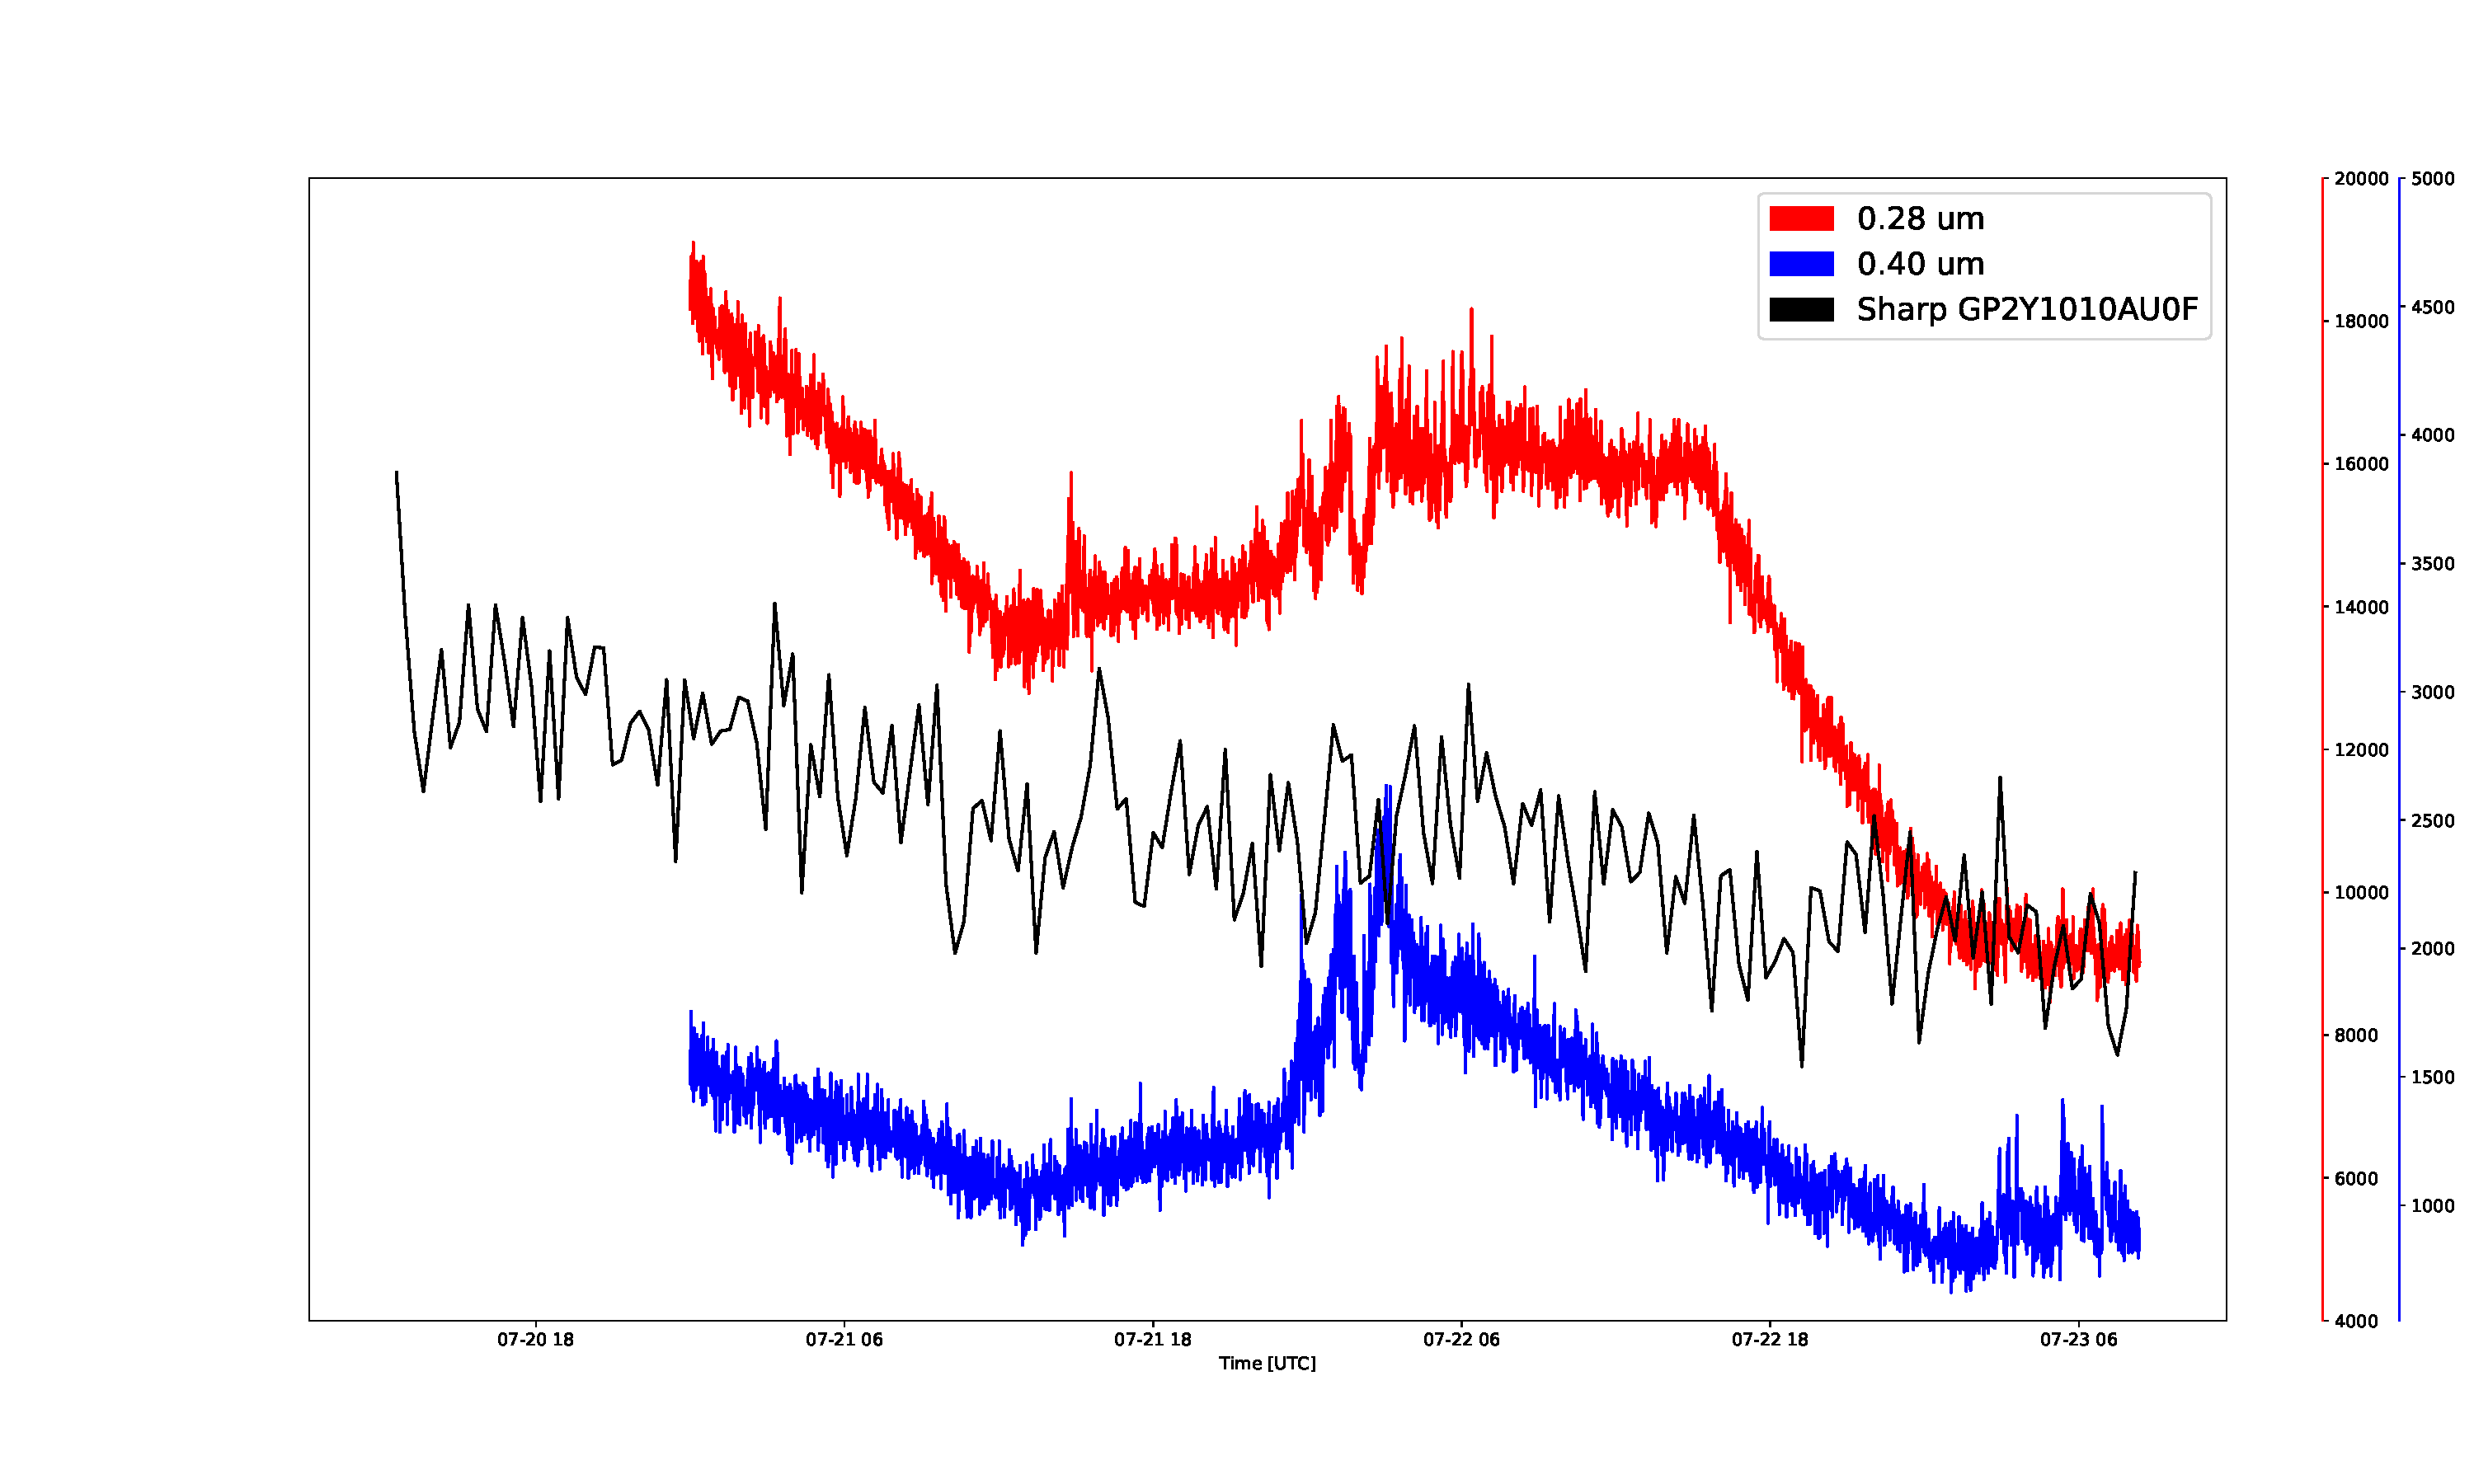
\includegraphics[width=16cm]{comparison.pdf}
		\caption{Primerjava meritev z referen"cnim tipalom}
		\label{comparison}
	\end{center}
\end{figure}

Za analizo uporabimo "se prej opisano metodo "stetja vrhov na posameznem intervalu. Program izpi"se tabelo \ref{table:correlations}, iz katere je razvidno, da z "stetjem vrhov na pravem intervalu dobimo korelacije, ki presegajo 0,9. To potrjuje tezoMeritve tipala Sharp GP2Y1010AU0F najbolje korelirajo z koncentracijami delcev velikosti med 0,25 in 0,50\,$\mu$m. 

\begin{table}[H]
	\centering
	\begin{tabular}{lll}
		velikost [$\mu m$] & korelacija & interval \\
		\hline
		0,25 & 0,94 & 68 - 72 \\
		0,28 & 0,94 & 68 - 72 \\
		0,30 & 0,93 & 68 - 72 \\
		0,35 & 0,93 & 76 - 84 \\
		0,40 & 0,96 & 76 - 84 \\
		0,45 & 0,91 & 76 - 84 \\
		0,50 & 0,91 & 80 \\
		0,58 & 0,74 & 80 \\
		0,65 & 0,39 & 80 \\
		0,70 & 0,30 & 48 \\
		0,80 & 0,34 & 48 \\
		1,00 & 0,44 & 48 \\
		1,30 & 0,50 & 52 \\
		1,60 & 0,59 & 52 \\
		2,00 & 0,70 & 52 \\
		2,50 & 0,71 & 52 \\
		3,00 & 0,66 & 52 \\
		3,50 & 0,67 & 64 \\
		4,00 & 0,68 & 64 \\
		5,00 & 0,68 & 64 \\
		6,50 & 0,68 & 64 \\
		7,50 & 0,68 & 64 \\
		8,50 & 0,68 & 64 \\
		10,00 & 0,68 & 64 \\
		12,50 & 0,67 & 64 \\
		15,00 & 0,66 & 64 \\
		17,50 & 0,66 & 64 \\
		20,00 & 0,66 & 64 \\
		25,00 & 0,66 & 64 \\
		30,00 & 0,66 & 64
		
	\end{tabular}
	\caption{Intervali korelacij pri primerjavi histogramske analize podatkov z referen"cnim tipalom}
	\label{table:correlations}
	\def\arraystretch{1}
\end{table}

\begin{figure}[H]
	\begin{center}
		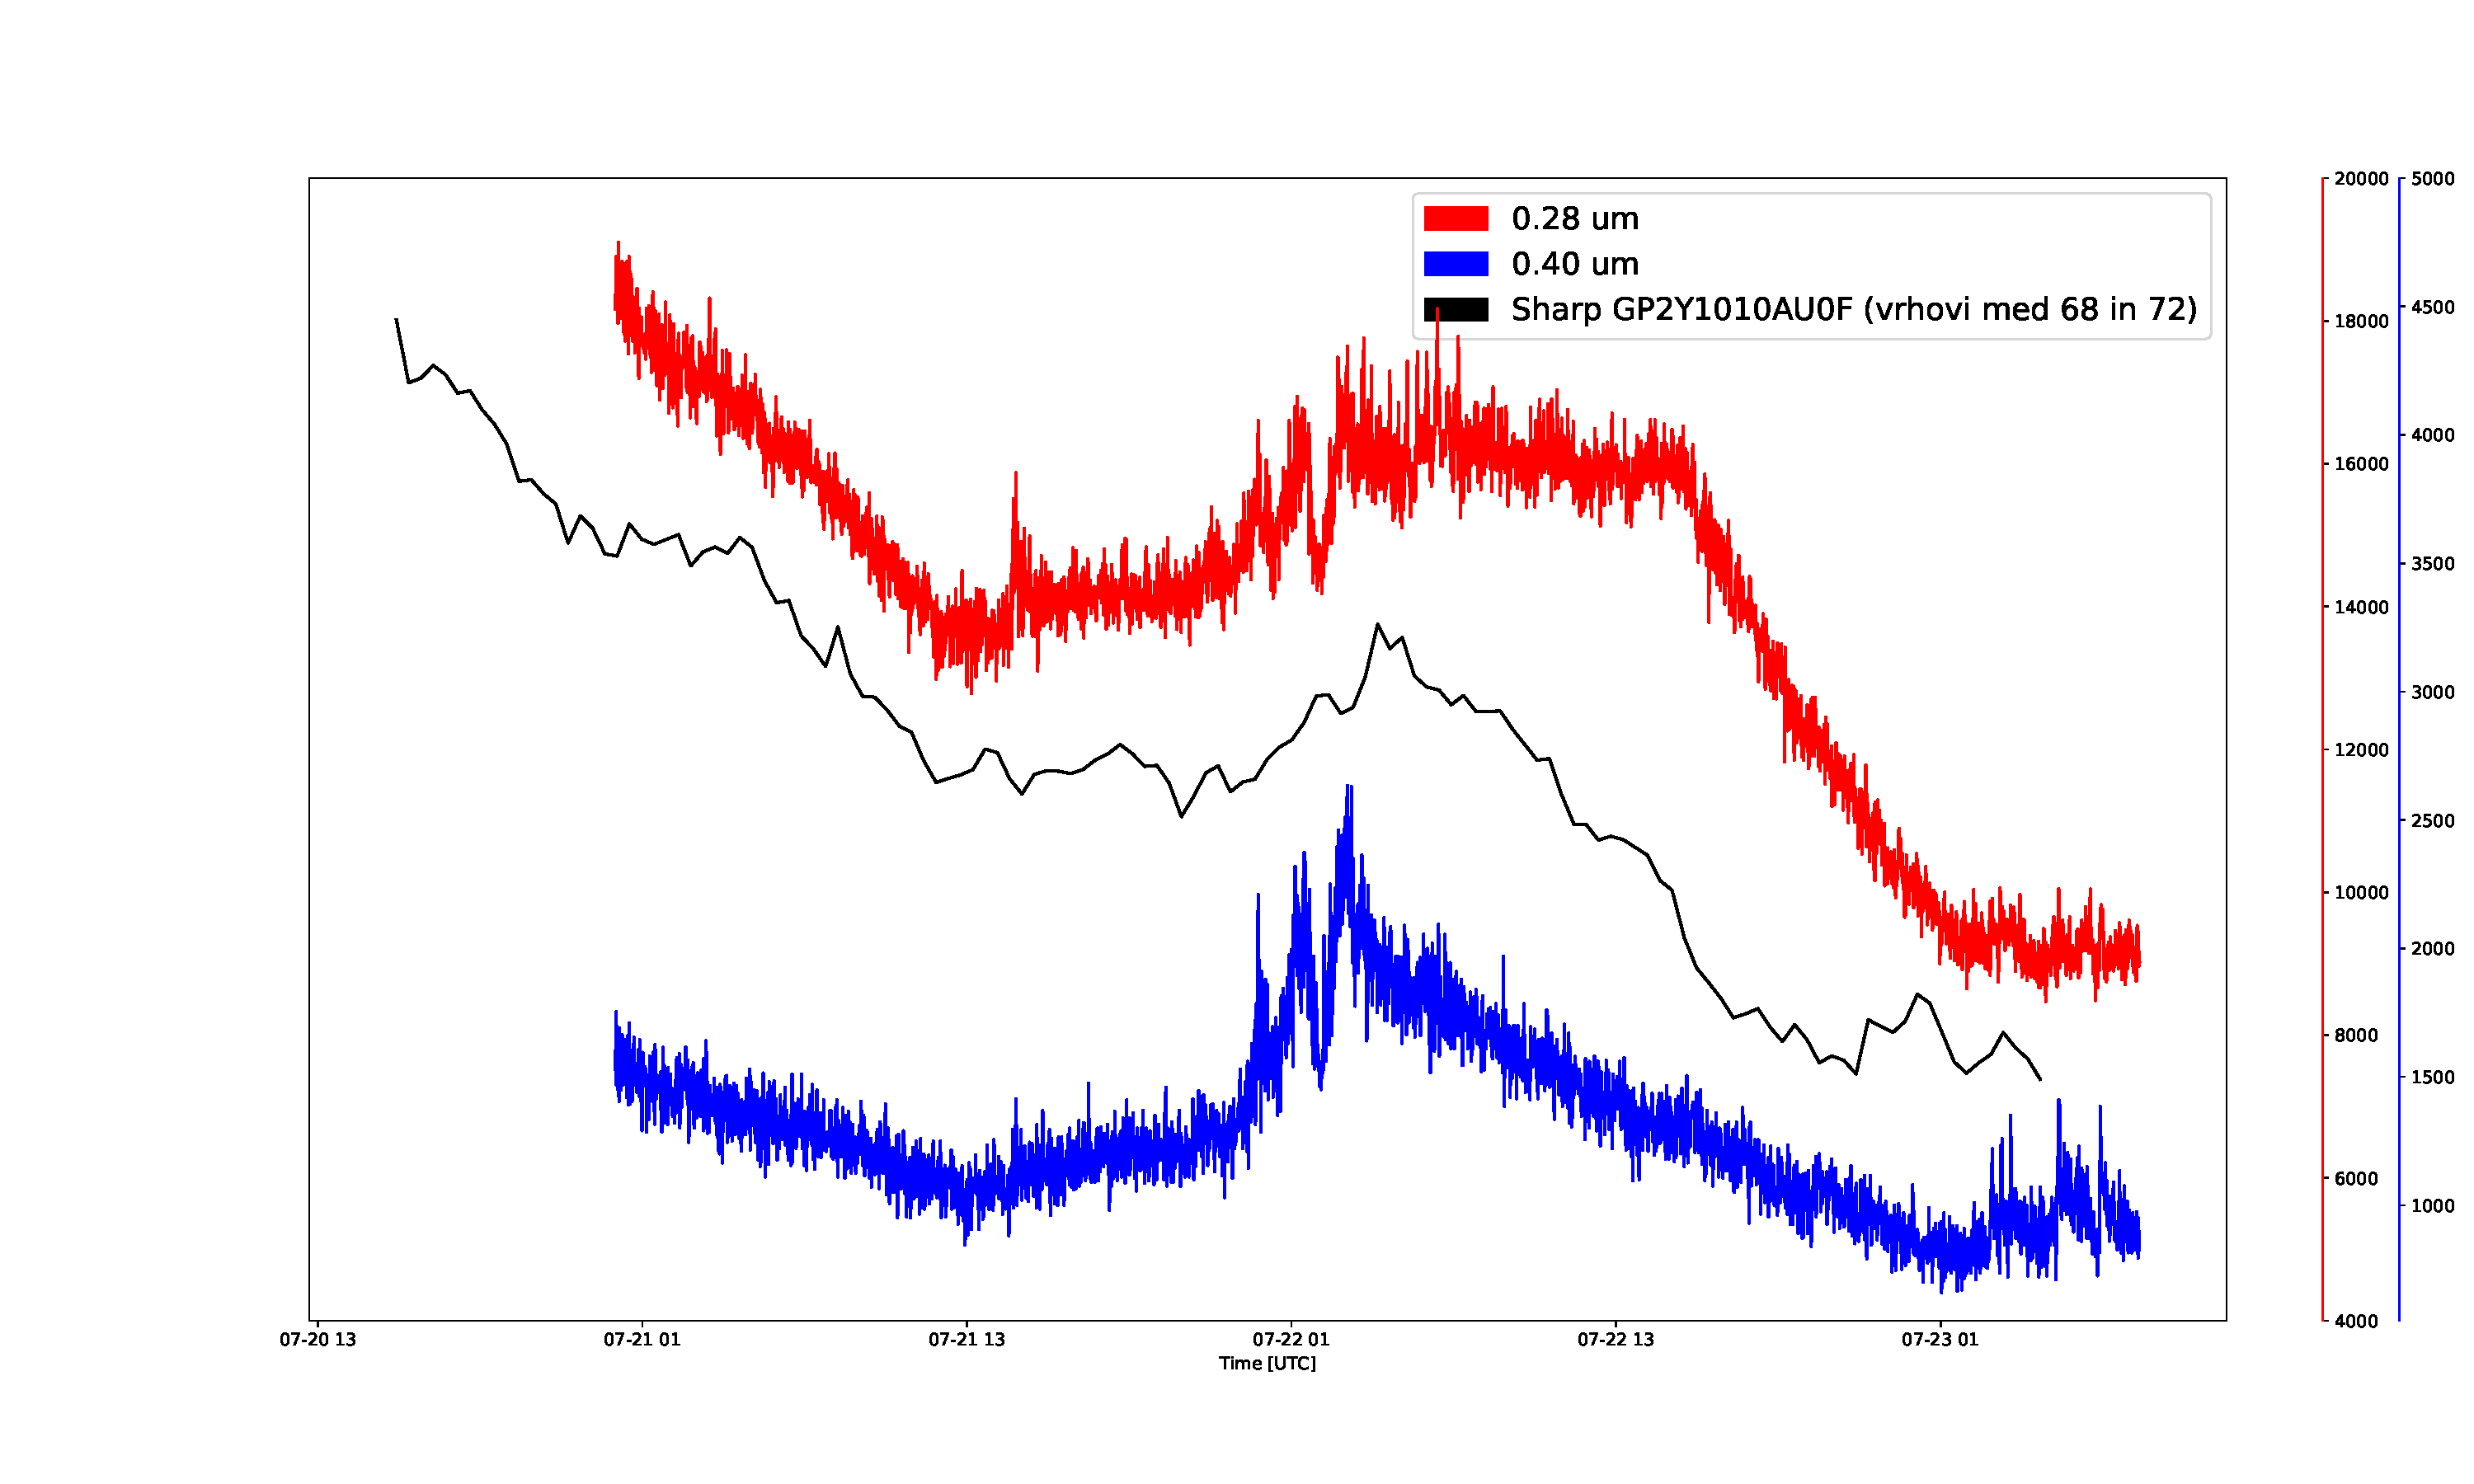
\includegraphics[width=16cm]{hist_comparison.pdf}
		\caption{Primerjava meritev z referen"cnim tipalom po histogramski analizi}
		\label{hist_comparison}
	\end{center}
\end{figure}

\clearpage

\begin{appendices}
	\section{Izvorna koda}
	\todo{potrebujem izvorno kodo kot prilogo?}
\end{appendices}
\clearpage

\section{Literatura}
\printbibliography[heading=none]
\end{document}